\documentclass[../monografia.tex]{subfiles}

\begin{document}
\section{Arquitetura da Rede}

\subsection{Conexão de Dispositivos}
Como citado anteriormente, as medições realizadas pelos dispositivos precisam ser salvas e enviadas para algum local de armazenamento, para posterior análise, exigindo que seja estabelecido um protocolo de conexão. 

Com o crescimento do conceito de Internet das Coisas, novas tecnologias para conexão rápida, segura e fácil de dispositivos são criadas e utilizadas por desenvolvedores em inúmeras aplicações. Segundo a pesquisa \textit{Embedded Markets Study} realizada pela empresa Aspencore\cite{embedded-market-study} e apresentada pelos meios EETimes\cite{eetimes} e Embedded\cite{embedded} em 2019, as interfaces sem fio mais utilizadas por desenvolvedores em  projetos de sistemas embarcados são Wi-Fi, \textit{Bluetooth Low Energy (BLE)} e \textit{Bluetooth Classic}. Essa pesquisa também aponta os protocolos de comunicação sem fio mais utilizados, dentre eles \textit{BLE mesh}, Zigbee, 6LoWPAN e Thread. 

Wi-Fi é uma família de tecnologias designadas para comunicação sem fio baseada no padrão IEEE 802.11\cite{802.11}, amplamente utilizada em redes de área local (em inglês \textit{local area network}, LAN) para prover acesso à internet como uma alternativa à tecnologia cabeada Ethernet. Essa tecnologia opera nas faixas de 2,4GHz e 5GHz, sendo que a primeira permite uma taxa de transmissão de até 600 Mbits/s e a segunda até 1 Gbit/s em casos mais extremos\cite{Wi-Fi-datarate}. A topologia comum de uma rede Wi-Fi é dada por um  dispositivo que atua como ponto de acesso que disponibiliza o sinal sem fio para que dispositivos ao seu redor possam se conectar à rede, em uma topologia de rede em estrela. Deste modo, os dispositvos têm que estar a uma distância de poucos metros do ponto de acesso para que a comunicação não seja afetada, sendo essa distância cerca de 76m a 122m em ambientes internos\cite{wifi-range}, dependendo da antena utilizada.

Outra norma comumente utilizada em redes sem fio é a IEE 802.15.4, que define especificações de camada física para redes de comunicação sem fio que operam com baixa taxa de transmissão de dados (em inglês, \textit{Lower Rate Wireless Personal Area Network,}, ou LR-WPAN), que também utiliza a banda de frequência de 2,4GHz\cite{802.15.4}. Os nós participantes da rede podem ser do tipo "função completa" (em inglês, \textit{full-function device} (FFD)), agindo como coordenador da rede, podendo retransmitir mensagens para outros nós, ou do tipo "função reduzida" (em inglês, \textit{reduced-function device} (RFD)), destinados a serem dispositivos simples e com poucos requisitos de comunicação, podendo apenas se comunicar com FFDs. As especificações Zigbee e 6LoWPAN são baseadas nessa norma.

Por último, dentre as tecnlogias citadas anteriormente, o Bluetooth surgiu com objetivo inicial de substituir a conexão por fios entre dispositivos móveis comuns como celulares e fones de ouvido, porém já evoluiu muito e pode ser encontrada em diversas aplicações. Em 2009, a \textit{Bluetooth Special Interest Group} (Bluetooth SIG, organização que gerencia o desenvolvimento do padrão Bluetooth) definiu uma nova versão de baixo consumo energético, chamada de \textit{Bluetooth Low Energy} (BLE), visando aplicações em que não é necessária comunicação contínua como, por exemplo, sensores que coletam dados em intervalos de tempo espaçados. O BLE vem se tornando uma das principais tecnologias para aplicações IoT, principalmente por estar presente na maioria dos dispositivos mais comuns utilizados no dia-a-dia das pessoas, como computadores, \textit{smartphones} e \textit{tablets}, o que facilita a comunicação do usuário com outros dispositivos específicos. As aplicações BLE operam a 2,4GHz com taxas de transmissão entre 0,27 e 1,37 Mbps\cite{ble-datarate}.

Os protocolos citados possuem, em geral, topologias de rede baseadas em estrela, com vários dispositivos periféricos conectados a um central, ou em árvore, que pode ser vista como várias redes em estrela interconectadas. No segundo caso, apenas os dispositivos centrais de cada rede em estrela poderia se comunicar com as outras, atuando como um dispositivo de borda. Desse modo, a conexão entre dispositivos periféricos e central da rede se dá de forma ponto-a-ponto, o que gera uma dependência forte do central e, caso ele apresente algum problema, pode afetar o funcionamento da rede inteira.


\begin{figure}[h!]
\centering
\begin{minipage}{.5\textwidth}
	\centering	
	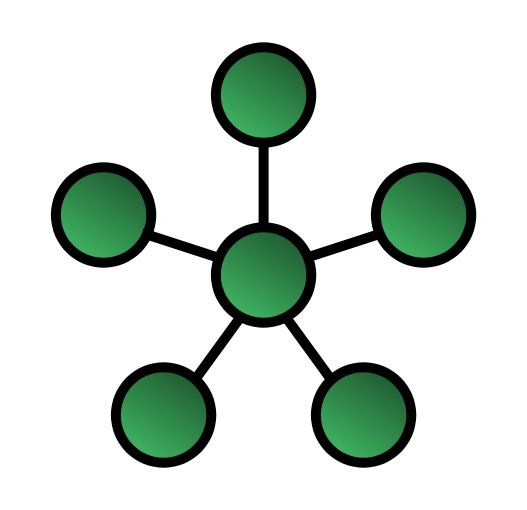
\includegraphics[width=.4\linewidth]{star-network}
	\caption{Topologia de rede em estrela}
	\label{fig:Rede em estrela}
\end{minipage}%
\begin{minipage}{.5\textwidth}
	\centering
	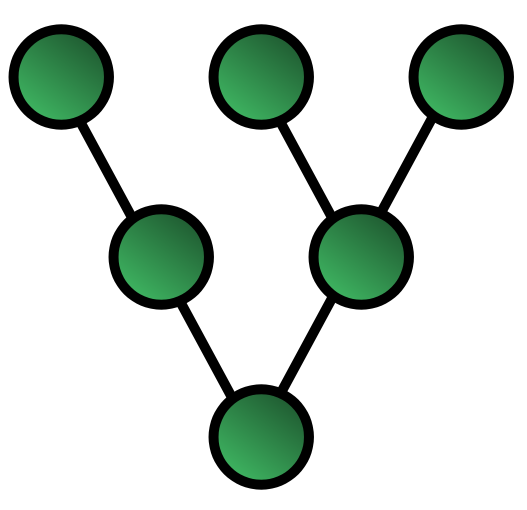
\includegraphics[width=.4\linewidth]{tree-network}
	\caption{Topologia de rede em árvore}
	\label{fig:Rede em árvore}
\end{minipage}

\end{figure}


O crescimento e evolução das aplicações IoT requer topologias mais novas e complexas, com a capacidade de se ajustarem dinamicamente caso ocorra alguma mudança na rede. Com isso em mente, soluções de redes em malha começam a surgir nos protocolos anteriormente citados. Nessa topologia, os nós ficam interligados de forma não-hierárquica, permitindo a comunicação \textit{many-to-many} entre os dispositivos da rede, possibilitando que dados de um ponto qualquer seja enviado a outro ponto qualquer da rede. 

\begin{figure}[h!]
\centering
	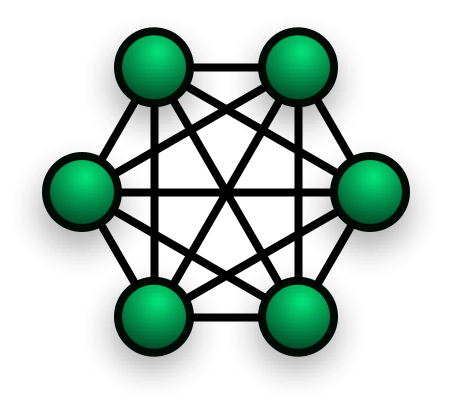
\includegraphics[width=.4\linewidth]{mesh-network}
	\caption{Topologia de rede em malha}
	\label{fig:Rede em malha}
\end{figure}

Dada essa necessidade, as epecificações dos protocos de comunicação começaram a adicionar soluções de rede em malha, como BLE Mesh, 802.11s (Wi-Fi mesh) e Thread, que é construída em cima da especificação 6LoWPAN. O protocolo Zigbee já possui suporte a redes em malha desde sua primeira concepção.

O artigo \textit{Wireless Mesh Networking: An IoT-Oriented Perspective Survey on Relevant Technologies}, publicado pela \textit{Future Internet}\cite{mesh-net-comparison} faz uma análise comparativa entre diferentes tipos de protocolos de comunicação atuando na topologia de rede em malha: família IEEE 802.15.4 (Zigbee e Thread), IEEE 802.11 (em especial a IEEE 802.11s que define redes em malha), LoRa Mesh e IEEE 802.15.4 (BLE Mesh). O protocolo LoRa foge do escopo deste projeto, pois é destinado para comunicações entre distâncias quilométricas, possui baixa taxa de transmissão de dados e consumo de energia muito elevado, como mostrado na imagem \ref{fig:Comparação redes mesh}.
 
CITAR ESTUDOS QUE COMPARAM ELAS, LIGANDO PRO GRÁFICO ABAIXO.


\begin{figure}[h!]
\centering
	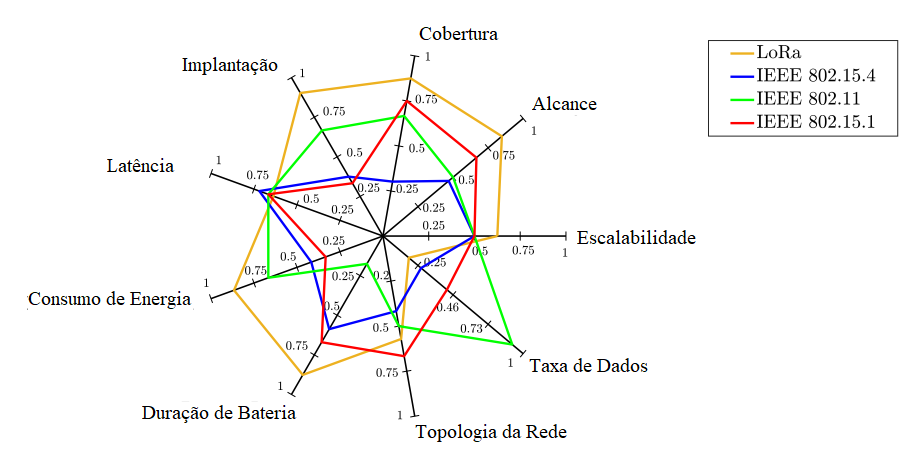
\includegraphics[width=\textwidth]{mesh-net-comparison}
	\caption{
		Comparação de performance entre 4 tecnologias de rede sem fio, em topologia de malha, de acordo com 9 parâmetros. Retirado de \cite{mesh-network-comparison} (traduzido).
	}
	\label{fig:Comparação redes mesh}
\end{figure}

Dados os requisitos desse projeto, os dispositivos serão interconectados por meio de uma rede \textit{Bluetooth Mesh}, disponibilizando dados de medições dos sensores e \textit{feedback} ao longo do dia por toda a rede. Um dos dispositivos da rede estará conectado também à internet via Wi-Fi, para que seja possível enviar os dados coletados pela rede para um banco de dados localizado em um servidor externo ao sistema, possibilitando o acesso remoto aos dados.


\subsection{Banco de Dados}
Outro requisito comumente encontrado em dispositivos IoT focados em monitoramento é a alta disponibilidade de dados para que esse monitoramento em questão seja realizado de forma eficiente. Isso faz com que soluções de armazenamento em nuvem sejam boas alternativas, já que os dados estariam armazenados em um servidor externo ao sistema, possibilitando o seu acesso remotamente. Grandes empresas de tecnologia oferecem plataformas de desenvolvimento com interfaces de programação de aplicações (API, do inglês \textit{application programming interface}) que facilitam o desenvolvimento de bancos de dados conectados.

Para esse projeto, usaremos a solução AWS da Amazon, especificamente o serviço \textbf{AWS IoT Core} \cite{aws-iot}, que é um serviço que permite conexão de dispositivos a aplicativos em nuvem. Ele será utilizado em conjunto com o banco de dados NoSQL DynamoDB da própria plataforma.


\section{Arquitetura do Dispositivo} % Como atingir os objetivos (requisitos) e apronfunda specs da descrição do problema (especificação inicial)
Nos nós da rede existirá um um dispositivo com a seguinte arquitetura:

\begin{figure}[h!]
    \centering
    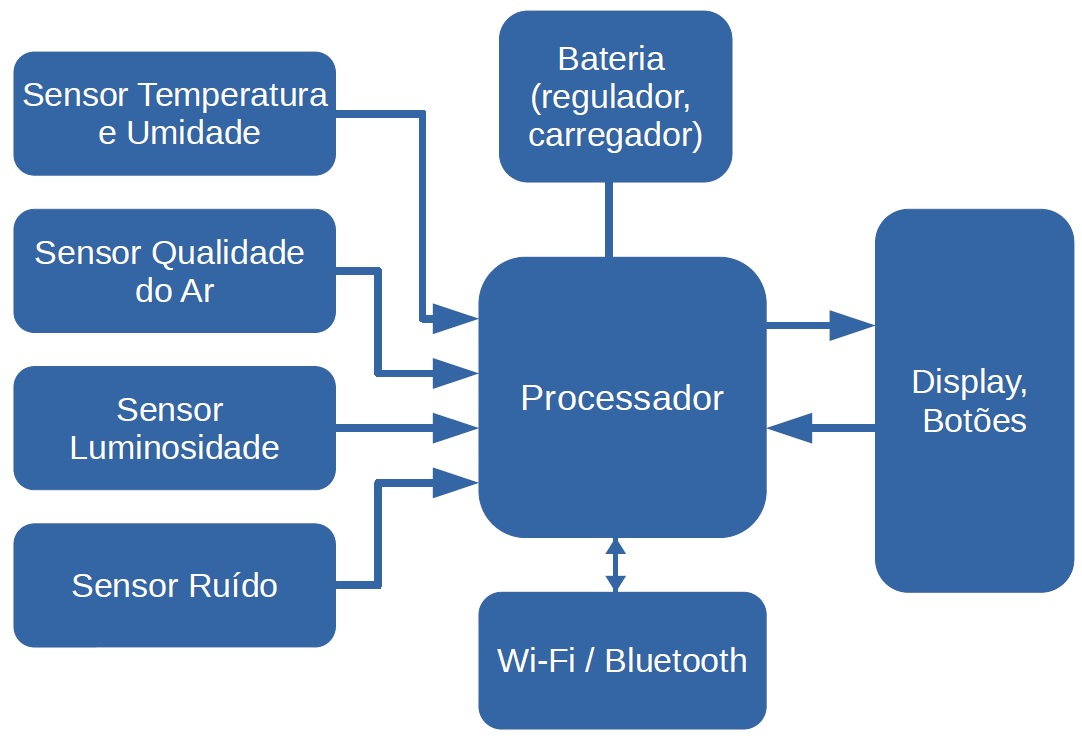
\includegraphics[width=10cm]{block_diagram}
    \caption{Diagrama de Blocos simplificado do dispositivo}
    \label{fig:Diagrama de Blocos}
\end{figure}

\subsection{Processador}

De acordo com a mesma pesquisa da Aspencore citada anteriormente, 61\% dos projetos de sistemas embarcados usam processadores de 32-bits, e 65\% utiliza algum tipo de sistema operacional. 

A partir da escolha de protocolos de comunicação e listando os periféricos necessários para comunicação com os periféricos (descritos a seguir), buscamos as principais opções existentes no mercado de microcontroladores para atuar como processador central do dispositivo. 

Como a comunicação dos dispositivos é uma funcionalidade crucial, juntamos as principais opções de \textit{System-on-a-Chip} (SoCs), ou Sistema em um chip. Estes tratam-se de circuitos integrados que englobam processadores (ou microcontroladores, usualmente em dispositivos embarcados), memórias, dentre outros módulos, como circuitos para comunicação sem fio, personalizados para uma aplicação \cite{soc}. Assim, chegamos a três opções de SoCs com Bluetooth integrado. 


\begin{center}
\begin{tabular}{|c|c|c|c|c|} 
\hline
\textbf{Vendor} & \textbf{Chip} & \textbf{Price} & \textbf{Kit} & \textbf{Kit Price} \\
\hline
Nordic Semi & BMD350 & \$11.3 & BMD350-EVAL & \$89 \\ 
Espressif Systems & ESP32 & \$3.8 & ESP32-DevKitC & \$10 \\ 
STMicroelectronics & BlueNRG-2 & \$3.5 & BlueNRG-Tile & \$50 \\ 
\hline
\end{tabular}
\end{center}

Analisando principalmente os ambientes de desenvolvimento, a documentação disponível e o preço dos CIs e de seus kits de desenvolvimento, optamos pela família ESP32 \cite{ESP32}. 

Além do Wi-fi como diferencial no SoC, a Espressif possui um bom suporte e ferramentas de desenvolvimento focadas em BLE e Wi-Fi, em especial para o uso de BLE Mesh, e um dos menores preços, assim considerado o melhor custo-benefício. 

\textbf{Especificações do ESP32:} \cite{ESP-datasheet}
\begin{itemize}
\item \textbf{Processador}: Xtensa 32-bits, dual core
\item \textbf{Wi-Fi}: 802.11 b/g/n
\item \textbf{Bluetooth}: v4.2 BR/EDR e BLE
\end{itemize}


\subsection{Sensores}
A fim de atender aos critérios apresentados para o monitoramento, foram escolhidos os seguintes sensores: 
\begin{itemize}
\item \textbf{AS7262}\cite{as7262}, da AMS: 

Atende aos requisitos de medição de \textit{conforto luminoso}. 

\textbf{Medidas}: Intensidade e cor da luz incidente.

A cor da luz, nesse sensor, é medida através de 6 canais, correspondendo aos espectros de luz vermelha (650nm), laranja (600nm), amarela (570nm), verde (550nm), azul (500nm) e violeta (450nm), ao invés de simples RGB, com resolução de 16 bits.

\textbf{Comunicação}: I²C, SPI ou UART (configurável)

\item \textbf{BME280} \cite{bme280}, da Bosch: 

Atende aos requisitos de \textit{conforto térmico}. 

\textbf{Medidas}: 
    \begin{itemize}
    \item Temperatura entre -40 e 85ºC, com precisão de ±1.0°C
    \item Umidade relativa com precisão de ±3\%
    \item Pressão entre 300 e 1100hPa, com precisão ±1 hPa
    \end{itemize}

\textbf{Comunicação}: SPI ou I²C

\item \textbf{SGP30} \cite{sgp30}:

Sensor para medições de aplicação \textit{indoor}. 

\textbf{Medidas}:
    \begin{itemize}
    \item TVOC entre 0 ppb e 60000 ppb, com resolução de 1ppb
    \item $CO_{2}$ entre 400 ppm e 60000 ppm, com resolução de 1ppb
    \end{itemize}

\textbf{Comunicação}: I²C

\item \textbf{Microfone de Eletreto}:

Em conjunto com um circuito amplificador, atende aos requisitos de \textit{conforto acústico}. 

\textbf{Medida}: volume de ruído sonoro ambiente

\textbf{Comunicação}: Analógica, precisão de 12 bits (resolução do conversor analógico-digital do ESP32). 
\end{itemize}

\subsection{Sistema de coleta de Feedback}

Para a coleta do \textit{feedback} nos dispositivos, optamos por utilizar um display e 2 botões. 

\subsection{Alimentação}

Para alimentar os dispositivos, foi pensado em utilizar uma bateria de Lítio-Polímero, de uma célula (1S), por ter a maior densidade energética dentre as baterias recarregáveis, permitindo que o dispositivo seja portátil e não dependente da rede elétrica. A capacidade da bateria será definida com base nos testes de consumo do equipamento nas etapas finais de desenvolvimento do protótipo. 

A bateria LiPo tem tensões de operação entre 3.5 e 4.2 Volts. Para alimentar o circuito foi optado por elevar a tensão para 5V, através de um regulador chaveado boost, ainda não definido. 

Para fazer a recarga da bateria de forma eficiente e segura, foi pensado em um circuito carregador utilizando o CI TP4056 \cite{tp4056}, alimentado por 5V através de um conector USB-micro. Com esse CI é possível também que o circuito opere enquanto a bateria está sendo recarregada. 


\end{document}
